
\section{Introduction}
\label{sec:introduction}

\noindent 
Almost every software system is subject to constant change due to evolving technology and user requirements. 
Its continuous development is largely driven by corrective, adaptive, perfective as well as preventive maintenance \cite{Lientz1980}.
The responsible development teams undergo changes as well and developers not involved in the previous development process are required to spent a considerable amount of their time understanding the system under maintenance. 
Furthermore, creating a mental model of a software is difficult, as it is virtual and intangible \cite{Knight2000}, thus, making it hard to communicate the structure and behavior of the system to decision makers. 
Visualization tools can provide communication artifacts such as software maps that assist software engineering and maintenance, \eg by allowing for actionable insights.

In recent years software maps were established to communicate static, dynamic, and evolutionary information of software systems as well as their software development processes by means of information visualization. 
The application of 2D or 3D map-oriented techniques constitute a fundamental approach in software visualization, software analytics, and software diagnosis.
Its primary applications include risk analysis for and monitoring of code quality, team activity, or software development progress \cite{Bohnet2011}.

\paragraph*{Evolution of Software Systems}
\noindent
The evolution of a software system can be tracked by, \eg revision control systems, making it possible to analyze changes over revision ranges by sampling revisions over time.
This information can be used for example to retrace, whether a design decision (\eg an architectural refactoring) resulted in an expected change that manifests itself in an improvement of respective \emph{software metrics}.
Existing approaches either use transition animations between multiple revisions to depict the evolution process or they convey a progress within a single static image:
Transition animations have the advantage of keeping the established metric mappings but do not scale for large software system or revision ranges with much change information to be displayed at once.
Conveying the characteristics of an evolution process within a static image does not suffer from this problem but existing approaches sacrifice at least one attribute mapping to encode an evolution measure.

\paragraph*{Metaphors for Trend Visualization}
\noindent
To overcome those shortcomings, a software map which uses natural phenomena as metaphors to visualize software metric trends within a static representation (\emph{trend map}) is used. 
In this paper, a static representation of the trend map denotes a visualization artifact that exhibits no transition animation with a revision range, but it can be explored using 3D interaction metaphors \cite{Jankowski2013}.
It combines the visualization of the static system structure with evolutionary information by augmenting interactive software maps with additional visual variables represented by natural phenomena (\eg fire, rain) or material properties (\eg rust, shininess, glow). 
Thereby, the visual variables that are used to depict the properties of the static system structure by mapping software metrics to color, area, and height can be maintained. 
Furthermore, the automatic computation of trends in metrics (\emph{metrics trends}) enables forecasting their future course, \eg increase, decrease, and stagnation. 
With the support of specific software metrics trends, decision makers can initiate preventive maintenance actions.

\begin{figure}[tbp]
	\centering
	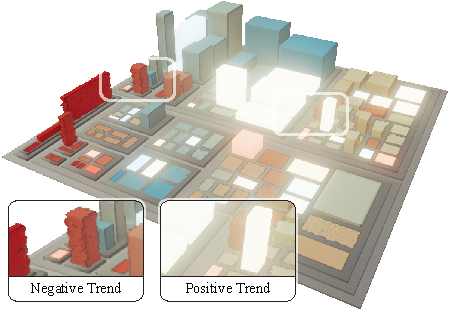
\includegraphics[width=\linewidth]{trendmap}
	\caption{
		This example depicts the trend of a system's test-coverage: 
		Area comprises lines-of-code, height relates to source code complexity, and color indicates test-coverage (red for lower and blue for higher coverage).
		Glowing items depict a positive trend, while a rough surface symbolizes a decrease in test-coverage during a specific time interval.}
	\label{fig:trendmap}
\end{figure}

When faced with unfamiliar concepts, our cognitive system searches for the best mapping between the unknown concept and existing knowledge of other domains \cite{Zhang2008}.
Software maps use a virtual city metaphor yielding a familiar 2.5D reference geometry. 
In this context, the application of natural phenomena as metaphors seems promising, since it can be assumed that they closely match to virtual 3D environments:
At best, their semantics are intuitively decoded making an additional legend non-obligatory. 
Examples of natural phenomena are objects aging in terms of their associated materials or degeneration within their environment (overgrown by grass, silted, gathering dust), changing in radiant emittance, as well as being exposed to natural forces such as fire, rain, wind, or sunshine (\autoref{fig:trendmap}).

\paragraph*{Challenges \& Contributions}
\noindent
A main challenge is the identification of natural phenomena that are suitable to effectively communicate trend data.
For it, metric values have to be mapped to parameters of respective rendering techniques in a comprehensive way. 
Furthermore, to extend their application to hierarchical structuring elements (\eg software modules) instead of individual leaf items only, hierarchical metric value aggregation is required. 
All in all, the challenges for an interactive visualization of trend data using natural phenomena as metaphors within software maps comprise
(1) a concept for mapping natural phenomena to software map items, 
(2) the aggregation of software metric values within revision ranges, 
(3) the metrics based parametrization of rendering techniques, and 
(4) rendering within real-time constraints.

With respect to these challenges, this paper contributes:
\begin{enumerate}

	\item A novel concept for the visualization of trend data within interactive software maps using natural phenomena.

	\item A technique for hierarchical aggregation of software system information and metrics automatically extracted from, \eg, revision control systems as well as a respective mapping to parametrize the real-time rendering techniques used for synthesis of natural phenomena.

	\item A prototypical implementation using the Unreal Engine 4 \cite{UnrealEngine4} capable of handling actual software system data.
	
\end{enumerate}

\noindent 
The remainder of this paper is structured as follows.
Related work \wrt interactive software visualization is reviewed in \autoref{sec:related}.
\autoref{sec:metaphors} presents a concept for trend visualization using item-based and context-based metaphors and \autoref{sec:design_and_parametrization} describes our hierarchical metric aggregation.
A prototype is briefly described in \autoref{sec:implementation} and demonstrated using actual software system data presented and discussed in \autoref{sec:results}. 
Finally, \autoref{sec:conclusions} concludes this work.
